\documentclass{article}
\usepackage{tikz}
\usetikzlibrary{automata,positioning}

\begin{document}

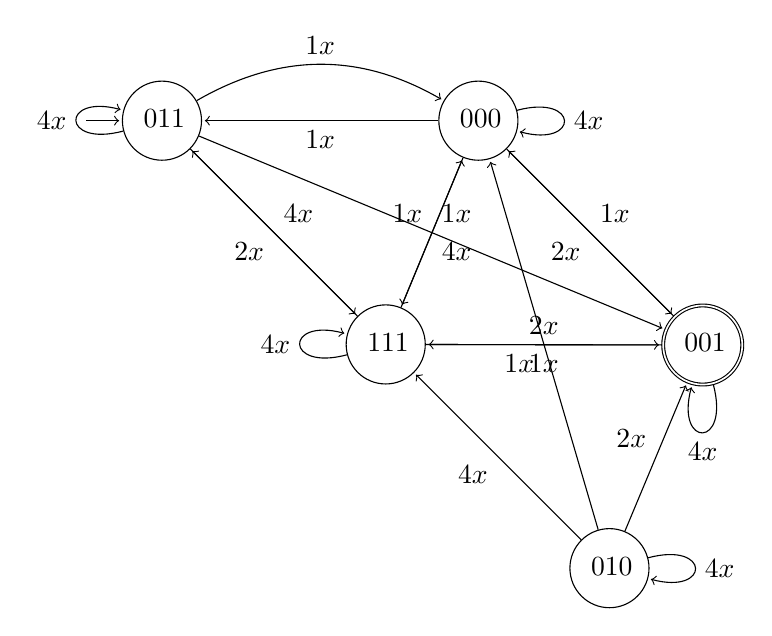
\begin{tikzpicture}[shorten >=1pt,node distance=3cm, initial text={}, auto]
    \node[state, initial] (q_0) {$\begin{matrix} 0 \\ 1 \\ 1 \end{matrix}$};
    \node[state] (q_1) [right=of q_0] {$\begin{matrix} 0 \\ 0 \\ 0 \end{matrix}$};
    \node[state] (q_2) [below right=of q_0] {$\begin{matrix} 1 \\ 1 \\ 1 \end{matrix}$};
    \node[state, accepting] (q_3) [below right=of q_1] {$\begin{matrix} 0 \\ 0 \\ 1 \end{matrix}$};
    \node[state] (q_4) [below right=of q_2] {$\begin{matrix} 0 \\ 1 \\ 0 \end{matrix}$};

    \path[->] 
    (q_0) edge [loop left] node {$4x$} ()
          edge [bend left] node {$1x$} (q_1)
          edge node {$4x$} (q_2)
          edge node {$1x$} (q_3);
    \path[->] 
    (q_1) edge [loop right] node {$4x$} ()
          edge node {$1x$} (q_0)
          edge node {$4x$} (q_2)
          edge node {$1x$} (q_3);
    \path[->] 
    (q_2) edge [loop left] node {$4x$} ()
          edge node {$2x$} (q_0)
          edge node {$1x$} (q_1)
          edge node {$2x$} (q_3);
    \path[->] 
    (q_3) edge [loop below] node {$4x$} ()
          edge node {$2x$} (q_1)
          edge node {$1x$} (q_2);
    \path[->] 
    (q_4) edge [loop right] node {$4x$} ()
          edge node {$1x$} (q_1)
          edge node {$4x$} (q_2)
          edge node {$2x$} (q_3);
\end{tikzpicture}

\end{document}